\documentclass[dvipdfmx]{jsarticle}
\usepackage{p2report}

\begin{document}

\maketitle


\begin{abstract}
    純粋な量子現象に重力が関わるものとして、COW効果が知られている。
    \cite{COWtheory}
    重力ポテンシャルが波動関数の位相に取り入れられ、2つの経路のビームを干渉させることで検出される。
    この現象はCollela, OverhauserとWernerによって単色熱中性子で検証された。
    \cite{COWexp}
\end{abstract}

\documentclass[dvipdfmx]{jsarticle}
\usepackage{p2report}

\begin{document}

\section{測定原理}


\subsection{中性子の干渉で発生する位相差}

% ideal COW
地上の中性子は重力ポテンシャルを受け、非相対論的にはHamiltonianが
\begin{equation*}
    H
    =
    \frac{\bm{p}^2}{2m}+mgz
\end{equation*}
となる。
$\bm{p}$は運動量、$m$は中性子質量、$g$は重力加速度でそれぞれ定数、$z$は基準面からの高さである。
中性子が弧長パラメーター$s$で表される軌道$\gamma(s)$を速さ$v(s)$で通過するとき、Schrödinger方程式の解は
\begin{equation*}
    \varphi
    =
    \exp[
        \frac{1}{i\hbar}\int\dd{t}
        \qty(
            \frac{\bm{p}^2}{2m}+mgz
        )
    ]
    =
    \exp[
        \frac{1}{i\hbar}\int_\gamma\frac{\dd{s}}{v}
        \qty(\frac{\bm{p}^2}{2m}+mgz)
    ]
\end{equation*}
の形で表される。
図\ref{fig: theoretical: neutron paths and O/H beams}のような経路を熱中性子が走る場合、中性子を波長$\lambda=h/mv$の単色平面波で近似すれば、面積$A$の平行四辺形での干渉によって点Eで位相差
\begin{equation}
    \label{eq: theoretical: delta phi g ideal}
    i\Delta\Phi_g
    :=
    i(\Phi_\mathrm{BCE}-\Phi_\mathrm{BDE})
    =
    \frac{mg}{i\hbar}
    \oint_\mathrm{BDEC}\dd{s}\frac{z}{v}
    =
    -i\frac{2\pi\lambda m^2gA}{h^2}\sin\delta
\end{equation}
が生じる。

\begin{figure}
    \centering
    \begin{tikzpicture}
        \draw[->, >=Stealth, dashed]($(-.3,0)+(-90:.3 and .5)$)arc(270:90:.3 and .5)node[above right]{$\delta$};
        \draw[->, >=Stealth](-1,0)node[left]{A}--(.5,0);
        \draw[dashed, preaction={line width=6pt, draw=white}]($(-.3,0)+(90:.3 and .5)$)arc(90:-90:.3 and .5);
        \draw(.5,0)--(1,0)node[below]{B};
        \draw(1,0)--++(.5,0);
        \draw(1.5,0)--(2,0)node[below right]{D};
        \draw[->, >=Stealth](2,0)--++(.5,.5);
        \draw(2.5,.5)--++(.5,.5)node[above left]{E};
        \draw[->, >=Stealth](3,1)--++(1,1)node[above right]{H beam};
        \draw[->, >=Stealth](1,0)--++(.5,.5);
        \draw(1.5,.5)--++(.5,.5)node[above left]{C};
        \draw(2,1)--++(.5,0);
        \draw[->, >=Stealth](2.5,1)--++(2,0)node[right]{O beam};
        \draw[->, >=Stealth](.5,1.)--++(0,.5)node[above]{$z$};
    \end{tikzpicture}
    \caption{
        中性子の経路。
        Oビーム、Hビームは共にA→B→D→E, A→B→C→Eの経路で進んだ中性子の干渉を反映する。
        ABを軸に全系を回転させると干渉が変化する。
        回転角度$\delta$は平行四辺形が水平面となす角で、図のように平行四辺形が鉛直面内にあってCEがBDよりも高い位置にあるとき$\delta=\pi/2$とする。
        $\delta=\pm\pi/2$とき干渉が最大で、$0$のときは干渉しない。
    }
    \label{fig: theoretical: neutron paths and O/H beams}
\end{figure}


% 平行度と位相差
四角形BDCEが平行四辺形から歪むと経路長や面積が変わって新たに位相差が生じる。
図\ref{fig: theoretical: alpha and paths}のようにギャップ$D$のエタロン2組が平行から相対角$\alpha$だけずれているとき、\eqref{eq: theoretical: delta phi g ideal}に現れる面積を四角形BDECで計算すると、
\begin{equation}
    \label{eq: theoretical: delta phi g}
    \Delta\Phi_g
    \simeq
    -\frac{2\pi m^2g}{h^2}
    \qty(
        2DL\cot2\theta
        -
        \frac{D^2}{2\sin^2\theta}\alpha
    )\lambda
\end{equation}
と近似される。
加えて経路長の変化により
\begin{equation}
    \label{eq: theoretical: delta phi a}
    \Delta\Phi_\alpha
    \simeq
    4\pi D\qty(
        \frac{1}{\lambda}
        -
        \frac{Nb_c}{2\pi\theta^2}\lambda
    )\alpha
\end{equation}
が現れる。
これは屈折率
\begin{equation*}
    n
    \simeq
    1-\frac{\lambda^2Nb_c}{2\pi}
\end{equation*}
による効果を表し、$N, b_c$はそれぞれ原子密度、中性子-原子核の散乱長である。
\cite{Fujiie_2024}
本実験の装置は$\alpha$を自由に変更することができ、$\alpha=0$に設定されている保証はない。
位相差は\eqref{eq: theoretical: delta phi g}と\eqref{eq: theoretical: delta phi a}の和
\begin{equation}
    \label{eq: theoretical: delta phi}
    \Delta\Phi
    =
    \Phi_\mathrm{BCE}
    -
    \Phi_\mathrm{BDE}
    =
    \Delta\Phi_g
    +
    \Delta\Phi_\alpha
\end{equation}
が実測される。

\begin{figure}
    \centering
    \begin{tikzpicture}
        \tikzmath{
            \tht=30;
            \alp=10;
            \D=0.5;
            \mirrorL=5;
        };
        \coordinate(full1)at(0,0);
        \coordinate(half11)at($(full1)+({-\D/tan(\tht)},\D)$);
        \coordinate(half12)at($(full1)+({\D/tan(\tht)},\D)$);
        \coordinate(full2)at($(half11)+(\tht:6)$);
        % mirrors
        \draw($(full1)+({-\mirrorL/2},0)$)--++(\mirrorL,0);
        \draw($(full1)+({-\mirrorL/2},\D)$)--++(\mirrorL,0);
        \draw($(full2)+({180-\alp}:{\mirrorL/2})$)--++(-\alp:{\mirrorL});
        \draw[name path=mirrorH2]($(full2)+({-90-\alp}:\D)+({180-\alp}:{\mirrorL/2})$)--++(-\alp:{\mirrorL});
        % beam 1
        \draw[very thick, name path=G1](half11)--(full2);
        % half 2 coordinate
        \path[name intersections={of= mirrorH2 and G1}];
        \coordinate(half21)at(intersection-1);
        \coordinate(half22)at($(half21)+(-\alp:{2*\D/tan(\tht)})$);
        % beam 2
        \draw[very thick, name path=G2](full1)--(half22);
        % other beams
        \draw[very thick](full1)--++({180-\tht}:3);
        \draw[very thick, name path=refF2, ->, >=Stealth](full2)--++({-\tht-2*\alp}:4)node[anchor=north]{O beam};
        \draw[very thick, ->, >=Stealth](half22)--++({-\tht-2*\alp}:3);
        \path[name intersections={of= mirrorH2 and refF2}, ->, >=Stealth];
        \draw[very thick, ->, >=Stealth](intersection-1)--++({\tht+\alp}:2)node[anchor=west]{H beam};
        \draw[very thick, ->, >=Stealth](half22)--++(\tht:2);
        % nodes
        \node at(full1)[anchor=north]{D};
        \node at(full2)[anchor=south]{C};
        \node at(half11)[anchor=south]{B};
        \node at(half12)[anchor=south]{I};
        \node at(half21)[anchor=north]{J};
        \node at(half22)[anchor=west]{K};
        \node at(intersection-1)[anchor=east]{L};
        \path[name intersections={of=refF2 and G2}];
        \node at(intersection-1)[anchor=north]{E};
        % values
        % \draw[dashed]($(half11)+({180-\tht}:1)$)arc({180-\tht}:180:1)node[anchor=south east]{$\theta$};
        \draw[dashed](full2)--++(-2,0)++(.5,0)arc(180:{180-\alp}:1.5)node[anchor=south]{$\alpha$};
        \draw[<->, >=Stealth]($(full2)+(0,1)$)node[anchor=center](P){}--($(full1)!(P)!($(full1)+(0,1)$)$)node[anchor=center](Q){};
        \node at($(P)!.5!(Q)$)[anchor=south]{$L$};
        \draw[<->, >=Stealth]($(full1)+({\mirrorL/2+0.25},0)$)--++(0,\D);
        \node at($(full1)+({\mirrorL/2+0.25},{\D/2})$)[anchor=west]{$D$};
    \end{tikzpicture}
    \caption{
        エタロンの相対角$\alpha$によるビーム経路(太線)の変化。
        $\alpha=0$のときに点E, K, Lが同一点になる。
        長さ$L$は1枚目のエタロンと平行に測ったエタロン間距離。
    }
    \label{fig: theoretical: alpha and paths}
\end{figure}


% 位相取り出し
B, C, D, E各点での反射や透過による位相の変化を考慮しても、上述の位相差を取り出せる。
図\ref{fig: theoretical: alignment and wave fnc}のような散乱体において入射、反射、透過の波動関数の間に
\begin{equation*}
    \mqty(\psi_o^1\\\psi_o^2)
    =
    \mqty(r & t \\ t' & r')
    \mqty(\psi_i^1\\\psi_i^2)
\end{equation*}
の関係があるとする。
確率の保存から行列はユニタリでなければならず、
\begin{equation}
    \label{eq: theoretical: unitary conditions of reflection and transparence}
    |r|^2
    =
    |r'|^2
    =
    1-|t|^2
    =
    1-|t'|^2
    ,\qquad
    r^\ast t+r't'^\ast
    =
    r^\ast t'+r't^\ast
    =0
\end{equation}
を満たす。
ハーフミラーと全反射ミラーはそれぞれ同一のものであるとして、それぞれに対応する行列を
\begin{equation*}
    \mqty(r & t \\ t' & r')
    ,\qquad
    \mqty(R & T \\ T' & R')
\end{equation*}
とすれば、点Bにて波動関数$\Psi_0$だったものは点Eにて
\begin{equation*}
    \begin{cases}
        \Psi_H
        =
        \Psi_0
        (
            r_\mathrm{B}t'_\mathrm{J}R_\mathrm{C}r'_\mathrm{L}
            e^{i\Phi_\mathrm{BCE}}
            +
            t'_\mathrm{B}R_\mathrm{D}t_\mathrm{I}t'_\mathrm{K}
            e^{i\Phi_\mathrm{BDE}}
        )
        \\
        \Psi_O
        =
        \Psi_0
        (
            r_\mathrm{B}t'_\mathrm{J}R_\mathrm{C}t_\mathrm{L}
            e^{i\Phi_{BCE}}
            +
            t'_\mathrm{B}R_\mathrm{D}t_\mathrm{I}r_\mathrm{K}
            e^{i\Phi_{BDE}}
        )
    \end{cases}
\end{equation*}
となる。
$|\Psi_0|^2=1$として\eqref{eq: theoretical: unitary conditions of reflection and transparence}を利用すると、ビーム強度は
\begin{equation*}
    \begin{cases}
        I_H
        =
        |R|^2|t|^2
        (
            |r|^4
            +|t|^4
            -2|r|^2|t|^2\cos(\Phi_\mathrm{BCE}-\Phi_\mathrm{BDE})
        )
        \\
        I_O
        =
        2|r|^2|R|^2|t|^4
        (1+\cos(\Phi_\mathrm{BCE}-\Phi_\mathrm{BDE}))
    \end{cases}
\end{equation*}
である。
ビーム強度は$\lambda$の関数として表されるので、
\begin{equation}
    \label{eq: theoretical: oscillation lambda}
    \mathscr{O}(\lambda)
    :=
    \frac{I_H-I_O}{I_H+I_O}
    =
    (|r|^2-|t|^2)^2-4|r|^2|t|^2\cos(\Delta\Phi)
\end{equation}
となり、$\lambda$と比較すれば、位相差$\Delta\Phi$を取得できる。

\begin{figure}
    \centering
    \begin{tikzpicture}
        \draw[ultra thick](-.75,0)--(.75,0);
        \draw[->, >=Stealth](150:1)node[above left]{$\psi_i^1$}--(150:.5);
        \draw[->, >=Stealth](-150:1)node[below left]{$\psi_i^2$}--(-150:.5);
        \draw[->, >=Stealth](-150:.5)--(30:1)node[above right]{$\psi_o^1$};
        \draw[->, >=Stealth](150:.5)--(-30:1)node[below right]{$\psi_o^2$};
    \end{tikzpicture}
    \caption{
        入射・反射・透過波の波動関数。
        上面を表とする。
    }
    \label{fig: theoretical: alignment and wave fnc}
\end{figure}


\subsection{多層膜ミラーの反射・透過特性}

多層膜ミラーの反射・透過率は1次元ポテンシャル問題として計算できる。
本研究で使用したミラーは\ref{fig: multilayer mirror}のようにガラスにTiとNiを積層しているものであり、それぞれ層の内部では中性子にoptical potentialがかかる。\cite{SekY:2011}
$V_i$と$k_i$を$i$番目の層におけるoptical potentialおよび波数の垂直成分、入射粒子の波数を$k$とすると、エネルギー保存から
\begin{equation*}
    k^2
    =
    k_j^2
    +
    \frac{2mV_j}{\hbar^2}
\end{equation*}
を得る。
$n_j^2:={k_j^2}/{k^2},\;\zeta:=kx$とすると、エネルギー$E$で入射した中性子のSchrödinger方程式は
\begin{equation*}
    \dv[2]{\Psi_j}{\zeta}
    =
    \frac{2m(V_j-E)}{\hbar^2k^2}\Psi_j(\zeta)
    =
    -n_j^2\Psi_j(\zeta)
\end{equation*}
と表せ、第$j$層と第$j+1$層の波動関数の間には
\begin{equation*}
    \mqty(\Psi_{j+1} \\ \Psi_{j+1}')
    =
    \mqty(
        \cos n_j\delta_j & n_j^{-1}\sin n_j\delta_j
        \\
        -n_j\sin n_j\delta_j & \cos n_j\delta_j
    )
    \mqty(\Psi_j \\ \Psi_j')
    =
    M_j
    \mqty(\Psi_j \\ \Psi_j')
\end{equation*}
の関係が成り立つ。
よって全ての層を通して
\begin{equation*}
    \mqty(\Psi_g \\ \Psi_g')
    =
    M
    \mqty(\Psi_0 \\ \Psi_0')
    \qquad
    \qty[
        M=M_N\cdots M_2M_1
        =
        \mqty(M_{11} & M_{12} \\ M_{21} & M_{22})
    ]
\end{equation*}
と書ける。
$\Psi_0=e^{ik\zeta_0}+Re^{-ik\zeta_0}, \Psi_g=Te^{ik(\zeta+\zeta_0)}$となる$R, T$を求めると、
\begin{equation}
    \label{eq: theoretical: R and T}
    \begin{split}
        R
        &=
        \frac{(M_{21}+ikM_{22})-ik(M_{11}+ikM_{12})}{ik(M_{11}-ikM_{12})-(M_{21}-ikM_{22})}
        \\
        T
        &=
        \frac{2e^{-ik\zeta}ik}{ik(M_{11}-ikM_{12})-(M_{21}-ikM_{22})}
    \end{split}
\end{equation}
を得る。

\begin{figure}
    \centering
    \begin{tikzpicture}
        \foreach \x in {0,1}
        {
            \draw(.2,{\x/2})rectangle(3.5,{\x/2+.25});
            \draw[fill=gray](.2,{\x/2+.25})rectangle(3.5,{\x/2+.5});
        }
        \node at(1.75,1.5)[anchor=center]{$\vdots$};
        \draw[->, >=Stealth, thick]($(1,0)!-.5!(2,1)$)--($(1,0)!1.5!(2,1)$);
        \draw[->, >=Stealth, thick](1.5,0)--($(1.5,0)!1.5!(2.5,1)$);
        \draw[->, >=Stealth, thick](2,0)--($(2,0)!1.5!(3,1)$);
        \draw[->, >=Stealth, thick](1,0)--++(.5,-.5);
        \draw[->, >=Stealth, thick](1.25,.25)--++(.75,-.75);
        \draw[->, >=Stealth, thick](1.5,.5)--++(1,-1);
        \draw[->, >=Stealth, thick](1.75,.75)--++(1.25,-1.25);
        \draw[->, >=Stealth, thick](2,1)--++(1.5,-1.5);
    \end{tikzpicture}
    \caption{多層膜ミラーの構造とビームの反射・透過。}
    \label{fig: multilayer mirror}
\end{figure}

これをもとに本研究で用いるミラーの反射率を入射角$\theta$, 波長$\lambda$ごとに計算すると、図\ref{fig: theoretical: reflectivity calculated}のようになった。
実験には反射率が安定して高い波長帯を与える入射角が望ましい。
\eqref{eq: theoretical: delta phi g}の角度依存性、使用する中性子ビームの波長帯も合わせて考慮し、本実験では$\theta=1.05^\circ$を採用した。

\begin{figure}
    \centering
    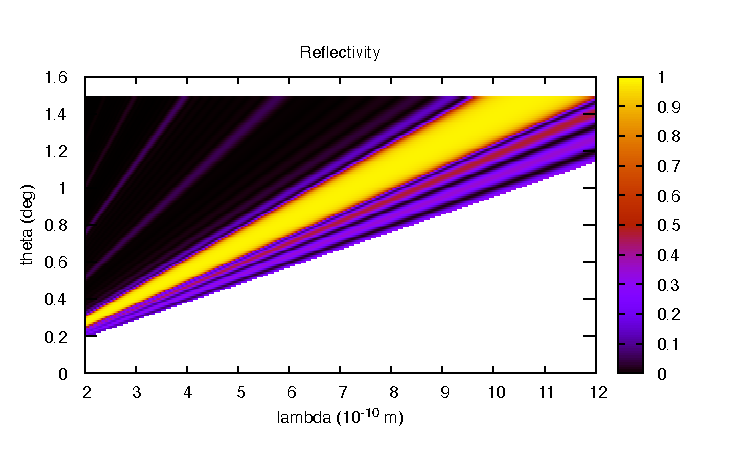
\includegraphics[width=8cm]{./img/reflNiTi2d.pdf}
    \caption{ミラーの反射率。計算にあたって\cite{SekY:2011}を参考にした。}
    \label{fig: theoretical: reflectivity calculated}
\end{figure}

\end{document}



\bibliographystyle{jplain}
\bibliography{bibbib}

\end{document}
